\documentclass[12pt, oneside]{article}

\usepackage[letterpaper, scale=0.8, centering]{geometry}
\usepackage{fancyhdr}
\setlength{\parindent}{0em}
\setlength{\parskip}{1em}

\pagestyle{fancy}
\fancyhf{}
\renewcommand{\headrulewidth}{0pt}
\rfoot{{\footnotesize Copyright Mia Minnes, 2024, Version \today~(\thepage)}}

\usepackage{titlesec}

\author{CSE105W24}

\newcommand{\instructions}{{\bf For all HW assignments:} Weekly homework 
may be done individually or in groups of up to 3 students. 
You may switch HW partners for different HW assignments. 
Please ensure your name(s) and PID(s) are clearly visible on the first page of your homework submission 
and then upload the PDF to Gradescope. If working in a group, submit only one submission per group: 
one partner uploads the submission through their Gradescope account and then adds the other group member(s) 
to the Gradescope submission by selecting their name(s) in the ``Add Group Members" dialog box. 
You will need to re-add your group member(s) every time you resubmit a new version of your assignment.
 Each homework question will be graded either for correctness (including clear and precise explanations and 
 justifications of all answers) or fair effort completeness. 
 For ``graded for correctness''
 questions: collaboration is allowed only with CSE 105 students in your group; 
 if your group has questions about a problem, you may ask in drop-in 
 help hours or post a private post (visible only to the Instructors) on Piazza.
 For ``graded for completeness''
 questions: collaboration is allowed with any CSE 105 students this quarter; 
 if your group has questions about a problem, you may ask in drop-in 
 help hours or post a public post on Piazza.

All submitted homework for this class must be typed. 
You can use a word processing editor if you like (Microsoft Word, Open Office, Notepad, Vim, Google Docs, etc.) 
but you might find it useful to take this opportunity to learn LaTeX. 
LaTeX is a markup language used widely in computer science and mathematics. 
The homework assignments are typed using LaTeX and you can use the source files 
as templates for typesetting your solutions.
To generate state diagrams of machines, we recommend using Flap.js
or JFLAP. Photographs of clearly hand-drawn diagrams may also be used. We recommend that you
submit early drafts to Gradescope so that in case of any technical difficulties, at least some of your
work is present. You may update your submission as many times as you'd like up to the deadline.


{\bf Integrity reminders}
\begin{itemize}
\item Problems should be solved together, not divided up between the partners. The homework is
designed to give you practice with the main concepts and techniques of the course, 
while getting to know and learn from your classmates.
\item You may not collaborate on homework questions graded for correctness with anyone other than your group members.
You may ask questions about the homework in office hours (of the instructor, TAs, and/or tutors) and 
on Piazza (as private notes viewable only to the Instructors).  
You \emph{cannot} use any online resources about the course content other than the class material 
from this quarter -- this is primarily to ensure that we all use consistent notation and
definitions (aligned with the textbook) and also to protect the learning experience you will have when
the `aha' moments of solving the problem authentically happen.
\item Do not share written solutions or partial solutions for homework with 
other students in the class who are not in your group. Doing so would dilute their learning 
experience and detract from their success in the class.
\end{itemize}

}

\newcommand{\gradeCorrect}{({\it Graded for correctness}) }
\newcommand{\gradeCorrectFirst}{\gradeCorrect\footnote{This means your solution 
will be evaluated not only on the correctness of your answers, but on your ability
to present your ideas clearly and logically. You should explain how you 
arrived at your conclusions, using
mathematically sound reasoning. Whether you use formal proof techniques or 
write a more informal argument
for why something is true, your answers should always be well-supported. 
Your goal should be to convince the
reader that your results and methods are sound.} }
\newcommand{\gradeComplete}{({\it Graded for completeness}) }
\newcommand{\gradeCompleteFirst}{\gradeComplete\footnote{This means you will 
get full credit so long as your submission demonstrates honest effort to 
answer the question. You will not be penalized for incorrect answers. 
To demonstrate your honest effort in answering the question, we 
expect you to include your attempt to answer *each* part of the question. 
If you get stuck with your attempt, you can still demonstrate 
your effort by explaining where you got stuck and what 
you did to try to get unstuck.} }

\usepackage{tikz}
\usetikzlibrary{automata,positioning,arrows}

\usepackage{amssymb,amsmath,pifont,amsfonts,comment,enumerate,enumitem}
\usepackage{currfile,xstring,hyperref,tabularx,graphicx,wasysym}
\usepackage[labelformat=empty]{caption}
\usepackage{xcolor}
\usepackage{multicol,multirow,array,listings,tabularx,lastpage,textcomp,booktabs}

% NOTE(joe): This environment is credit @pnpo (https://tex.stackexchange.com/a/218450)
\lstnewenvironment{algorithm}[1][] %defines the algorithm listing environment
{   
    \lstset{ %this is the stype
        mathescape=true,
        frame=tB,
        numbers=left, 
        numberstyle=\tiny,
        basicstyle=\rmfamily\scriptsize, 
        keywordstyle=\color{black}\bfseries,
        keywords={,procedure, div, for, to, input, output, return, datatype, function, in, if, else, foreach, while, begin, end, }
        numbers=left,
        xleftmargin=.04\textwidth,
        #1
    }
}
{}

\newcommand\abs[1]{\lvert~#1~\rvert}
\newcommand{\st}{\mid}

\newcommand{\cmark}{\ding{51}}
\newcommand{\xmark}{\ding{55}}


\newcommand{\SUBSTRING}{\textsc{Substring}}
\newcommand{\REP}{\textsc{Rep}}
\newcommand{\blank}{\scalebox{1.5}{\textvisiblespace}}


\title{HW1 : Regular Expressions and Finite Automata}
\date{Due: April 11th at 5pm (no penalty late submission until 8am next morning), via Gradescope}


\begin{document}
\maketitle
\thispagestyle{fancy}


{\bf In this assignment,}

You will practice reading and
applying the definitions of alphabets, strings, languages, Kleene star, and regular expressions.
You will use regular expressions and relate them to languages and finite automata.
You will use precise notation to formally define the state diagram of finite automata,
and you will use clear English to describe computations of finite automata informally.


{\bf Resources}: To review the topics 
for this assignment, see the class material from Week 1.
We will post frequently asked questions and our answers to them in a 
pinned Piazza post.

{\bf Reading and extra practice problems}: Sipser Section 0, 1.3, 1.1.
Chapter 1 exercises 1.1, 1.2, 1.3, 1.18, 1.23.

\instructions

You will submit this assignment via Gradescope
(\href{https://www.gradescope.com}{https://www.gradescope.com}) 
in the assignment called ``hw1CSE105Sp23''.

{\bf Assigned questions}
%%%%%%%%%%% PROBLEM 1 %%%%%%%%%%%

\begin{enumerate}[wide, labelwidth=!, labelindent=0pt]
    \item \textbf{Functions over sets of strings} (17 points): \\
    For this question, fix the alphabets $\Sigma = \{0,1\}$ and
    $\Gamma = \{0,1,2\}$.

    Whenever $K$ is a set of strings over $\Gamma$ and 
    $L$ is a set of strings over $\Sigma$, 
    we can use the following 
    rules to define associated sets of strings:
    \begin{align*}
    \SUBSTRING(K) &:= \{ w \in \Gamma^* \mid \text{there exist } a,b \in \Gamma^* \text{ such that } awb \in K\} \\
    \REP(L) &:= \{ w \in \Gamma^* \mid \text{between every 
    pair of successive $2$s in $w$ is a string in $L$}\}\\
    &\phantom{:}=\{w \in \Gamma^* \mid \text{for all } v \in \Sigma^* \text{ if } 2v2 \in \SUBSTRING(\{w\})  \text{, then } v \in L\}
    \end{align*}
    \textit{Note:} Formally, $\SUBSTRING$ and $\REP$ are functions
    whose domains and codomains are specified as
    $$\SUBSTRING: \mathcal{P}(\Gamma^*) \to \mathcal{P}(\Gamma^*)$$ 
    and 
    $$\REP: \mathcal{P}(\Sigma^*) \to \mathcal{P}(\Gamma^*)$$
    In other words, $\SUBSTRING$ maps sets of strings with characters $\{0,1,2\}$ to associated
    sets of strings with characters $\{0,1,2\}$; and $\REP$ maps sets of strings with characters 
    in $\{0,1\}$ to associated sets of strings with characters in $\{0,1,2\}$.
    \begin{enumerate}
    \item \gradeCorrectFirst Consider $w = 0120$ (which is a string in $\Gamma^*$). 
    List every element of the set $\SUBSTRING(\{w\})$. 
    In other words, fill in the blank
    \[
    \SUBSTRING(\{w\}) = \{ \underline{\phantom{\hspace{3in}}} \}
    \]
    Briefly justify your answer by referring back to the relevant definitions.

    {\it Not graded, but good to think about: Why do we need the curly braces---``$\{$'' and ``$\}$''---around $w$ for the input to $\SUBSTRING$?}

    \item\gradeCorrect Specify an example language $A$ over $\Gamma$ such that 
    $A \neq \Gamma^*$ and yet $\SUBSTRING(A) = \Gamma^*$, 
    or explain why there is no such example. 
    A complete solution will include either (1) a precise and
    clear description of your example language $A$ 
    and a precise and clear description of
    the result of computing $\SUBSTRING(A)$ using relevant definitions 
    to justify this description and to justify the set equality with 
    $\Gamma^*$, or (2) a sufficiently general and correct argument
    why there is no such example, referring back to the relevant definitions.

    \item\gradeCompleteFirst Define the language $B$ to 
    be the language over $\Sigma$ described by the regular expression 
    \[
    \Sigma^* 1 \Sigma^*
    \] 
    In plain English, we might explain that $B$ is the set of all 
    strings of $0$s and $1$s that contain a $1$. Give a plain English 
    explanation for the set of strings $\REP(B)$.
    
    \item\gradeCorrect Prove/disprove:
    For every finite language $L$ over $\Sigma$, $\REP(L)$ is also a finite
    set of strings.  A complete answer will either give a general
    argument starting with an arbitrary finite language and proving 
    that the result of applying $\REP$ is also finite, or will give a 
    counterexample (which is a specific example of a finite language 
    $L$ for which applying $\REP$ gives an infinite language, with 
    justification referring back to the relevant definitions).

    {\it Note: A finite language is a set of finitely many strings. 
    This includes the possibility that $L$ is the empty set!}

    \item\gradeComplete Write a template for a regular expression that describes $\REP(L)$
    when $L$ is described by a regular expression $R$.
    You may use union, concatenation, Kleene star, and 
    $\Sigma$, $\Gamma$, and $R$.  (We're using the shorthand for regular expressions
    describing alphabets from page 64.)

    \end{enumerate}

%%%%%%%%%%% PROBLEM 2 %%%%%%%%%%%
    \item \textbf{Deciphering regular expressions} (22 points): \\
    For this question, let's fix the regular expression over the alphabet $\{0,1\}$
    \[
    R = 0^* (1 \cup 10)^*
    \]

    For each choice of strings of length $3$, 
    $a, b, c \in \{0,1\}^3$ we can define the regular
    expression:
    \[
    X_{a,b,c} = 0 (a \cup b \cup c)^* 
    \]
    \begin{enumerate}
    \item \gradeComplete Give a plain English explanation for the language 
    described by the regular expression $R$. 
    This continues a theme from Problem~1---before trying to prove formal statements about a specific regular expression, it's often 
    good to try to translate it into a form that is more easy to reason about. 
    Typically speaking, the shorter and more concise your plain English 
    description is, the more useful it will be in reasoning about the language.
        
    \item \gradeCorrect Suppose $a = 000$, $b=001$, $c=011$ so 
    \[
    X_{a,b,c} = 0 ( 000 \cup 001 \cup 011)^*
    \]
    Show that $L(R) \not\subseteq L(X_{a,b,c})$ by giving some string in $L(R)$ 
    which is not in $L(X_{a,b,c})$, and justifying this choice referring back to relevant definitions.

    \item \gradeCorrect More generally, prove that 
    \[
    L(R) \not\subseteq L(X_{a,b,c})
    \]
    for \emph{all} possible strings $a, b, c \in \{0,1\}^3$. 
    Hint: What are the possible lengths of strings in $L(R)$ (and why does this help)?

    \item \gradeCorrect Give 
    a specific example of three distinct strings $a, b, c \in \{0,1,2\}^3$ such that 
    \[
    L(X_{a,b,c}) \subseteq L(R)
    \]
    Briefly justify your answer by 
    explaining how an arbitrary element of $L(X_{a,b,c})$ is guaranteed to be an element of 
    $L(R)$.

    \item \gradeCorrect Give a specific 
    example of three distinct strings $a, b, c \in \{0,1,2\}^3$ such that 
    \[
    L(X_{a,b,c}) \not\subseteq L(R)
    \]
    Briefly justify your 
    answer by giving a counterexample string 
    that is in $L(X_{a,b,c})$ and is not in $L(R)$
    (and explaining why using relevant definitions).
    \end{enumerate}

%%%%%%%%%%% PROBLEM 3 %%%%%%%%%%%
    \item \textbf{The right transition function can make or break a DFA} (6 points): \\
    Consider the finite automaton $(Q, \Sigma, \delta, q_0, F)$ depicted below
    \begin{center}
    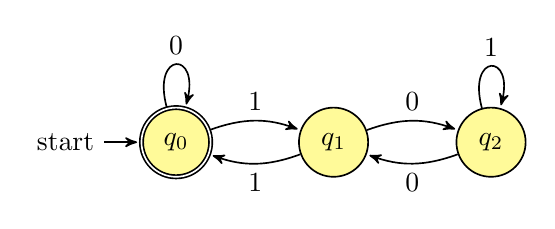
\begin{tikzpicture}[->,>=stealth',shorten >=1pt, auto, node distance=2cm, semithick]
    \tikzstyle{every state}=[text=black, fill=yellow!40]

    \node[initial,state, accepting] (q0)                    {$q_0$};
    \node[state]         (q1) [right of=q0] {$q_1$};
    \node[state]         (q2) [right of=q1] {$q_2$};

    \path (q0) edge  [loop above] node {$0$} (q0)
            edge [bend left=20] node {$1$} (q1)
        (q1) edge [bend left=20] node {$0$} (q2)
            edge [bend left=20] node {$1$} (q0)
        (q2) edge [loop above] node {$1$} (q2)
            edge [bend left=20] node {$0$} (q1)
    ;
    \end{tikzpicture}
    \end{center}
    where $Q = \{q_0, q_1, q_2\}$, $\Sigma = \{0,1\}$, and $F = \{q_0\}$. 

    \begin{enumerate}
    \item \gradeComplete Find and fix the mistake in the 
    following symbolic description of the transition function $\delta \colon Q \times \Sigma \to Q$: for each $j \in \{0,1\}$
    \[
    \delta(q_0, j) = q_j \hspace{2cm} \delta(q_1, j) = q_{1-j} \hspace{2cm} \delta(q_2, j) = q_{1+j}
    \]
    \item \gradeCorrect Keeping the same set of states $Q = \{q_0, q_1, q_2\}$, alphabet $\Sigma = \{0,1\}$, starting state $q_0$, and set
    of accepting states $F = \{q_0\}$, change the transition function $\delta$ so that the resulting finite
    automaton recognizes the language 
    described by the regular expression
    \[
        0^* \cup \Sigma^* 1000^*
    \]
    Briefly justify why the resulting finite automaton works 
    by describing the role of each state with your new transition function and relating it to a plain English description 
    of the language described by the regular expression.

    Note: with regular expressions $*$ binds more tightly than concatenation 
    so $1000^* = (100)(0^*)$.

    \end{enumerate}
    {\it (Challenge question, not graded) There is a beautiful plain English description of the language recognized by the finite automaton
    with the state diagram depicted at the start of Problem~3. 
    What is it?}

    %%%%%%%%%%% PROBLEM 4 %%%%%%%%%%%
    \item \textbf{Being precise with terminology} (5 points): \\
    For each of the following statements, determine if 
    it is true, false, or if the question doesn't even 
    make sense (because the statement isn't well formed
    or doesn't use terms in ways consistent with definitions from class).

    \begin{enumerate}
    \item\gradeComplete The empty string is in every language.
    \item\gradeComplete $\Sigma^*$ is a language.
    \item\gradeComplete Every language is a regular expression.
    \item\gradeComplete Alphabets are infinite.
    \item\gradeComplete There is a (finite) number $k \in \mathcal N$ such that every DFA has fewer than $k$ states.
    \end{enumerate}
\end{enumerate}
\end{document}